\DiaryEntry{Huffman Codes, cont'd}{2021-05-03}{Coding}

\subsection{Code Performance}

To demonstrate the performance of Huffman codes, I created a script which creates an alphabet with given size and random symbol probabilities. \todo{add ref}

For $N = 8$ symbols and $10.000$ runs, the mean source entropy is $H \approx 2.736$ bits and the average code word length $l \approx 2.789$. The average difference between code word length and source entropy divided by the source entropy equals $\approx 0.01965$; i.e. we are $2\%$ away from the optimum. The minimum code word length is $1$ bit and maximum code word length is $7$ bits.

The picture is similar for $N = 32$ symbols: Mean source entropy is $H \approx 4.724$ bits and the average code word length $l \approx 4.757$. The average difference between code word length and source entropy divided by the source entropy equals $\approx 0.006845$; i.e. we are $0.6\%$ away from the optimum. The minimum code word length is $3$ bit and maximum code word length is $12$ bits.

The Huffman code procedure assigns short code words (e.g. $1$ bit) only when the symbol probability is very high. It seems that this happens very seldom in the simulation; If we manually tilt the symbol probability of the first symbol to higher values, then we get a minimum code word length of $1$.

As a fun fact, we also note that if we run the Huffman coding procedure with $N = 2^l$ symbols ($l$ being an arbitrary integer) and equal probabilities $1/N$, it produces a "normal" binary code with all symbols having $l$ bits.

\subsection{Canonical Huffman Codes}

It is useful to develop Huffman codes which can be stored in an efficient manner. One way to do this is to write the code in lexicographic order of the symbols. Thus, we first write the code for $a_1$ , then the code for $a_2$, and so on. Each codeword could be represented by the length of the codeword followed by the codeword. 

For the code in Table \ref{2021-04-14_tab1}, we therefore would have $[1, 4, 0001, 2, 4, 0000, 3, 3, 001, \\ 4, 2, 01,  5, 1, 1]$.

This is certainly manageable for the Huffman code of a small alphabet, but it is clearly going to have an impact on compression performance when we have Huffman codes for large alphabets.

We can substantially reduce the storage requirement for the code by using a version of the Huffman code known as the \emph{canonical Huffman code}. We first examine a property of Huffman trees: A Huffman tree is a fully populated tree. That is, there is a codeword assigned to each leaf of the tree (if a codeword is shorter than the longest codeword, the tree below the codeword is pruned; see the previous entry, \ref{2021-04-26:entry}). What we will show is that if we are only given the lengths of the codewords moving from left to right on the tree we can reconstruct the code.

In our running example, the Huffman code has codeword lengths $[4, 4, 3, 2, 1]$. In order to regenerate the code from the lengths, we begin with a tree of depth four (the length of the longest codeword), as shown in the following Figure.

\begin{figure}[H]
    \centering
    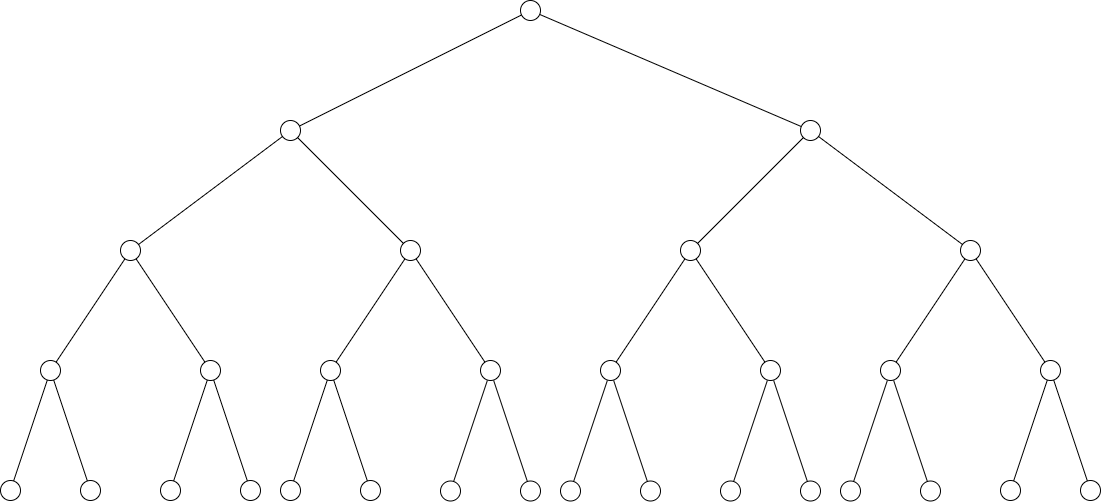
\includegraphics[scale=0.4]{images/2021-05-03_tree_01.png}
\end{figure}


The first codewords have length $4$ so they are located all the way down in the tree. The next codeword has length $3$, so we choose the next "free" node in the tree with length $3$. A Huffman code is a prefix code, we therefore have to prune all nodes below codeword $3$. For the codeword of length $2$ we again choose the next "free" node of length $2$ and prune everything below. Finally, we do the same for the last codeword with length $1$. The resulting tree looks as follows.

\begin{figure}[H]
    \centering
    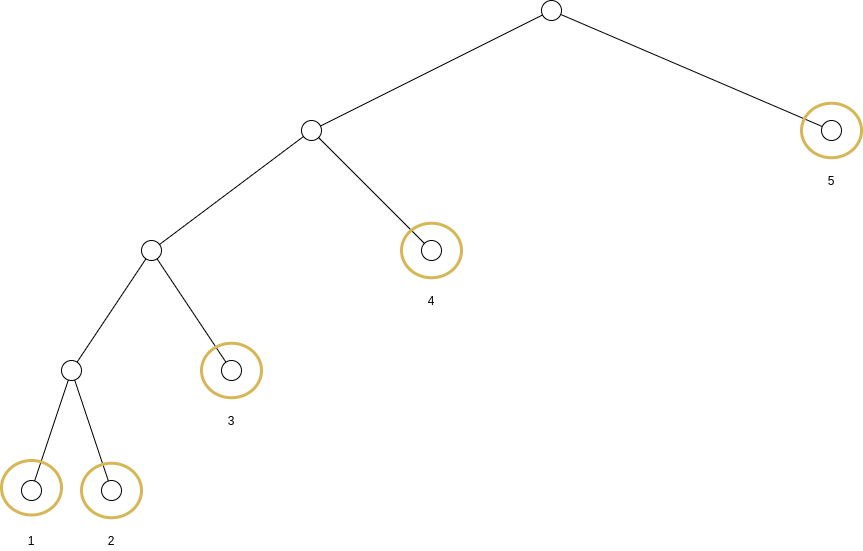
\includegraphics[scale=0.4]{images/2021-05-03_tree_02.png}
\end{figure}

If we assign the left subtree a $1$ and the right subtree a $0$, then we can recover the original code tree and corresponding codewords.So, just knowing the codeword lengths in a particular order permits us to regenerate the Huffman code. The problem is that we do not know which codeword belongs to which letter. The canonical procedure provides us with a way to generate a code that implicitly contains that information. In order to embed this additional information, we need some additional constraints to our Huffman coding procedure. For example, the deflate algorithm in zlib imposes the following conditions on a Huffman code:

\begin{itemize}
    \item All codes of a given length have lexicographically consecutive values in the same order as the symbols they represent.
    \item Shorter codes lexicographically precede longer codes.
\end{itemize}

 Recall that when we generated Huffman codes, we could choose to assign zeros and ones to the branches as we wished. These constraints can be viewed as taking that freedom away.

 We can incorporate these constraints into the Huffman coding procedure, or we can generate a Huffman code using the procedure described previously and transform the code thus produced into a canonical Huffman code. It is simpler to use the latter approach. In order to do this, we will begin by designing a Huffman code. From this design, we will extract the lengths of the codewords. We will use these lengths with the canonical constraints to design the code.

Our example consists of $5$ symbols, $\{a_1, a_2, a_3, a_4, a_5\}$ with codeword lengths $\{4,4,3,2 \\,1\}$. The shortest codeword is assigned to $a_5$, the lexicographically smallest codeword of length one is $0$, so the codeword for $a_5$ is $0$. The codeword of length two has to be of the form $1x$. Since we require only one codeword of length two, we assign $10$ to $a_4$. The codewords of length three now have to be of the form $11x$. We only need a single codeword of length three, the codeword for $a_3$; therefore, the codeword for $a_3$ is $110$. There are two codewords, $a_4$ and $a_5$, of length 4. Therefore, the codeword for $a_4$ is $1110$, and the codeword for $a_5$ is $1111$.

This code can now be encoded by just sending the symbols and their codeword lengths; the actual codewords are \emph{not} required. The resulting codetree is shown in the following Figure.

\begin{figure}[H]
    \centering
    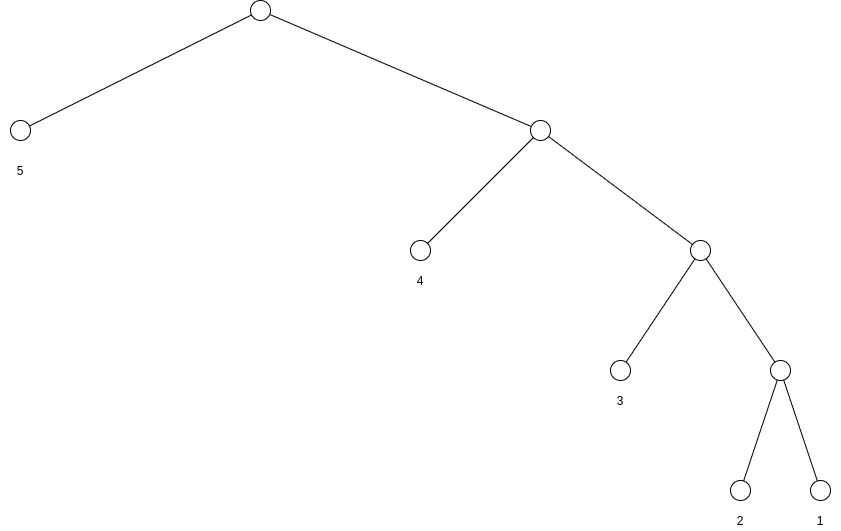
\includegraphics[scale=0.4]{images/2021-05-03_tree_03.png}
\end{figure}


\subsection{Length-limited Huffman Codes}

The Huffman coding algorithm tries to minimize the average length of codewords. However, there are no limits on the maximum length of an individual codeword. This is not necessarily a problem when dealing with limited alphabet sizes. However, if the alphabet size is relatively large there is a possibility of getting very long Huffman codes. This can be avoided by adding an additional constraint to the variable length code design problem: a requirement that all codewords be less than or equal to some maximum codeword length $l_{max}$. If $m$ is the size of the source alphabet, then clearly $l_{max}$ has to be greater than or equal to $\lceil \log_2 m \rceil$ for the code to be a valid code.

The most widely used algorithm for constructing length-limited Huffman codes is the package-merge algorithm due to Larmore and Hirschberg. We will use a couple of facts from our prior discussions to design length limited Huffman codes. First, all we need to obtain a Huffman code is the length of the codewords. Second, for an alphabet of size $m$, the lengths of the codewords $l_1 , l_2, \ldots, l_m$ in any variable length code have to satisfy the Kraft–McMillan inequality 

\bee
\sum_i 2^{-l_i} \leq 1
\eee

and, given a set of $l_i$ which satisfy the Kraft–McMillan inequality, we can always find a uniquely decodable code with codewords of length $l_i$.

For the following, we assume our alphabet consists of the letters $a_1, a_2, \ldots , a_m$ with probabilities $p_1, p_2, \ldots, p_m$. We will assume that the letters have been sorted based on their probabilities $p_i$; i.e. $p_i$ is the smallest probability and $p_m$ the largest.

The design process will involve incrementing the lengths $l_i$ until the Kraft–McMillan inequality is satisfied while at the same time keeping the average length $\bar{l}$ as small as we can. We start with assigning zero bits for all lengths. Clearly, this will result in the lowest possible length of zero. However, it certainly does not give us a uniquely decodable code; for fun, we can check with the Kraft–McMillan inequality as

\bee
\sum_i 2^{-l_i} = \sum_i 2^{0} = m \nleq 1
\eee

We can decrement this sum by $0.5$ by incrementing the codeword for one of the letters to one. We want to pick the codeword which will have the minimal impact on the average codeword length. As the letters are sorted in nondecreasing probability order and the average codeword length is given by $\sum_i l_i p_i$, we will increase $l_1$ by one. This will give us an average codeword length of $p_1$ ($1 \times p_1 + 0 \times p_2 + \cdots = p_1$) and a Kraft–McMillan sum of $m - 0.5$. Actually, we could have picked any of the letters as we will need to increment each length to at least one if we are to have any hope of reducing the Kraft–McMillan sum to one. However, once we have incremented each codeword length to one how do we decide which codeword lengths to increment further? The package merge algorithm is an iterative algorithm which solves this problem by generating a list of choices which can be sorted in order of increasing cost.

Each iteration consists of two steps operating on the list, a packaging step and a merge step. In the packaging step the list from the previous step is partitioned, or packaged, into groups of two neighboring items. The cost of a package is the sum of the costs of the items in the package where the cost of a letter is the probability of that letter. If the number of items is odd the item with the highest cost is discarded. In the merge step the packages from the previous step are merged with the list of items that consists of the individual letters. This list is then sorted in order of increasing cost. After $l_{max} - 1$ iterations the lowest cost $2m - 2$ items are selected. Each time an item contains a letter results in the incrementing of the codeword for that letter by one. As there are $2m-2$ items each of which decrements the Kraft–McMillan sum by $0.5$ we end up with a set of lengths $l_i$ such that

\bee
\sum_i 2^{- l_i} = 1 \qed
\eee

\paragraph{Example.} Let us design a length-limited Huffman code for a source with five sybmols. Symbol probabilities are as follows: $P(a_1) = 0.05, P(a2) = 0.1, P(a3) = 0.15, P(a4) = P(a5) = 0.2, P(a6) = 0.3$. The entropy for this source is $2.409$ bits/symbol. Using the standard Huffman procedure we can generate a code 
as follows (taken from the book, own implementation yields different bits but the same average length):

\vspace{3mm}

\begin{tabular}{cc|c}
    Symbol & Probability & Codeword \\ \hline
    $1$ & $0.05$ & $0100$ \\
    $2$ & $0.1$ & $0101$ \\
    $3$ & $0.15$ & $011$ \\
    $4$ & $0.2$ & $10$ \\
    $5$ & $0.2$ & $11$ \\
    $6$ & $0.3$ & $00$
\end{tabular}

\vspace{3mm}

with an average length $\bar{l} = 2.45$. The longest codewords are four bits long. Let us design a code with the added constraint that $l_{max} = 3$.

We begin with the list of letters. The costs are listed next to the letters,

\bee
[a_1(0.05), a2(0.1), a3(0.15), a4(0.2), a5(0.2), a6(0.3)]
\eee

We then proceed with the first packaging step. The packages are denoted by $a_{jk}(p)$ where the subscripts indicate the letters in the package and the quantity $p$ in the argument is the total cost of the item. In the first packaging step we form packages by grouping the letters two-by-two to form Package 1:

\bee
[a_{12}(0.15), a_{34}(0.35), a_{56}(0.5)]
\eee

We then merge these packages with our original list to get the merged list (ordered by cost; i.e. probability)

\bee
[a_1(0.05), a2(0.1), a3(0.15), a_{12}(0.15), a4(0.2), a5(0.2), a_6(0.3), a_{34}(0.35), a_{56}(0.5)]
\eee

To get a code limited to three bits we need to go through one more iteration. In the next packaging step we take the items in the previous merged list and group them two-by-two to yield Package 2,

\bee
[a_{12}(0.15), a_{312}(0.3), a_{45}(0.4), a_{634}(0.65)]
\eee

Finally, we go through one more merge operation in which we merge the packages with the original list of letters to obtain Merge 2,

\begin{align*}
    [& a_1(0.05), a2(0.1), a3(0.15), a_{12}(0.15), a4(0.2), a5(0.2), a6(0.3), \\ & a_{312}(0.3), a_{34}(0.35), a_{45}(0.4), a_{56}(0.5), a_{634}(0.65)]    
\end{align*}


We now pick the ten items ($2m-2 = 2 \cdot 6 - 2 = 10$) with the lowest cost and count the number of times each letter appears in the ten items. The letter $a_1$ appears in $a_1$ , $a_{12}$ , and $a_{312}$. Therefore, the number of bits in the codeword for $a_1$ is three. Continuing in this fashion we obtain the lengths of the codewords as $\{3, 3, 3, 3, 2, 2\}$. A code with these lengths is as follows,

\vspace{3mm}

\begin{tabular}{cc|c}
    Symbol & Probability & Codeword \\ \hline
    $1$ & $0.05$ & $100$ \\
    $2$ & $0.1$ & $101$ \\
    $3$ & $0.15$ & $110$ \\
    $4$ & $0.2$ & $111$ \\
    $5$ & $0.2$ & $00$ \\
    $6$ & $0.3$ & $01$
\end{tabular}

\vspace{3mm}

The average codeword length is $2.5$ bits; that's $0.05$ bits worse than the Huffman code obtained previously. \qed

%%% Local Variables:
%%% mode: latex
%%% TeX-master: "journal"
%%% End:
